% Lecture 05 How to write the SRS Sep 2021 Complete: https://docs.google.com/document/d/1fnwYnqAYdEQx13KpmQvulktGNpjKAKfx/edit
% Lecture 05 MSc Project - How to write the SRS Chapter: https://docs.google.com/document/d/1lEheSmKF9sDZkRozLTLSJ8XBDC_4yDxL/edit

% 2. We critically evaluated the Chapter 4 of the sample thesis - https://drive.google.com/drive/folders/1GlPK41lsmaZ26HIwK64AFwvb-3u0Chpx?usp=sharing (Visit Chapter 04 of the thesis and see my comments to see how you can improve)

% --------------

\section{Chapter Overview}
This chapter focuses on identifying possible stakeholders of the project by taking a look at all possible points of interaction with the system with the use of a rich picture diagram, gathering their perceptions to analyse and come up with possible expected use cases, functional and non-functional requirements of the prototype. 

\section{Rich Picture}

% rich picture in canva: https://www.canva.com/design/DAEwtvMqut8/k-BGnDBlelk824WGuNdb7g/edit

\begin{figure}[h!]
\centering
\frame{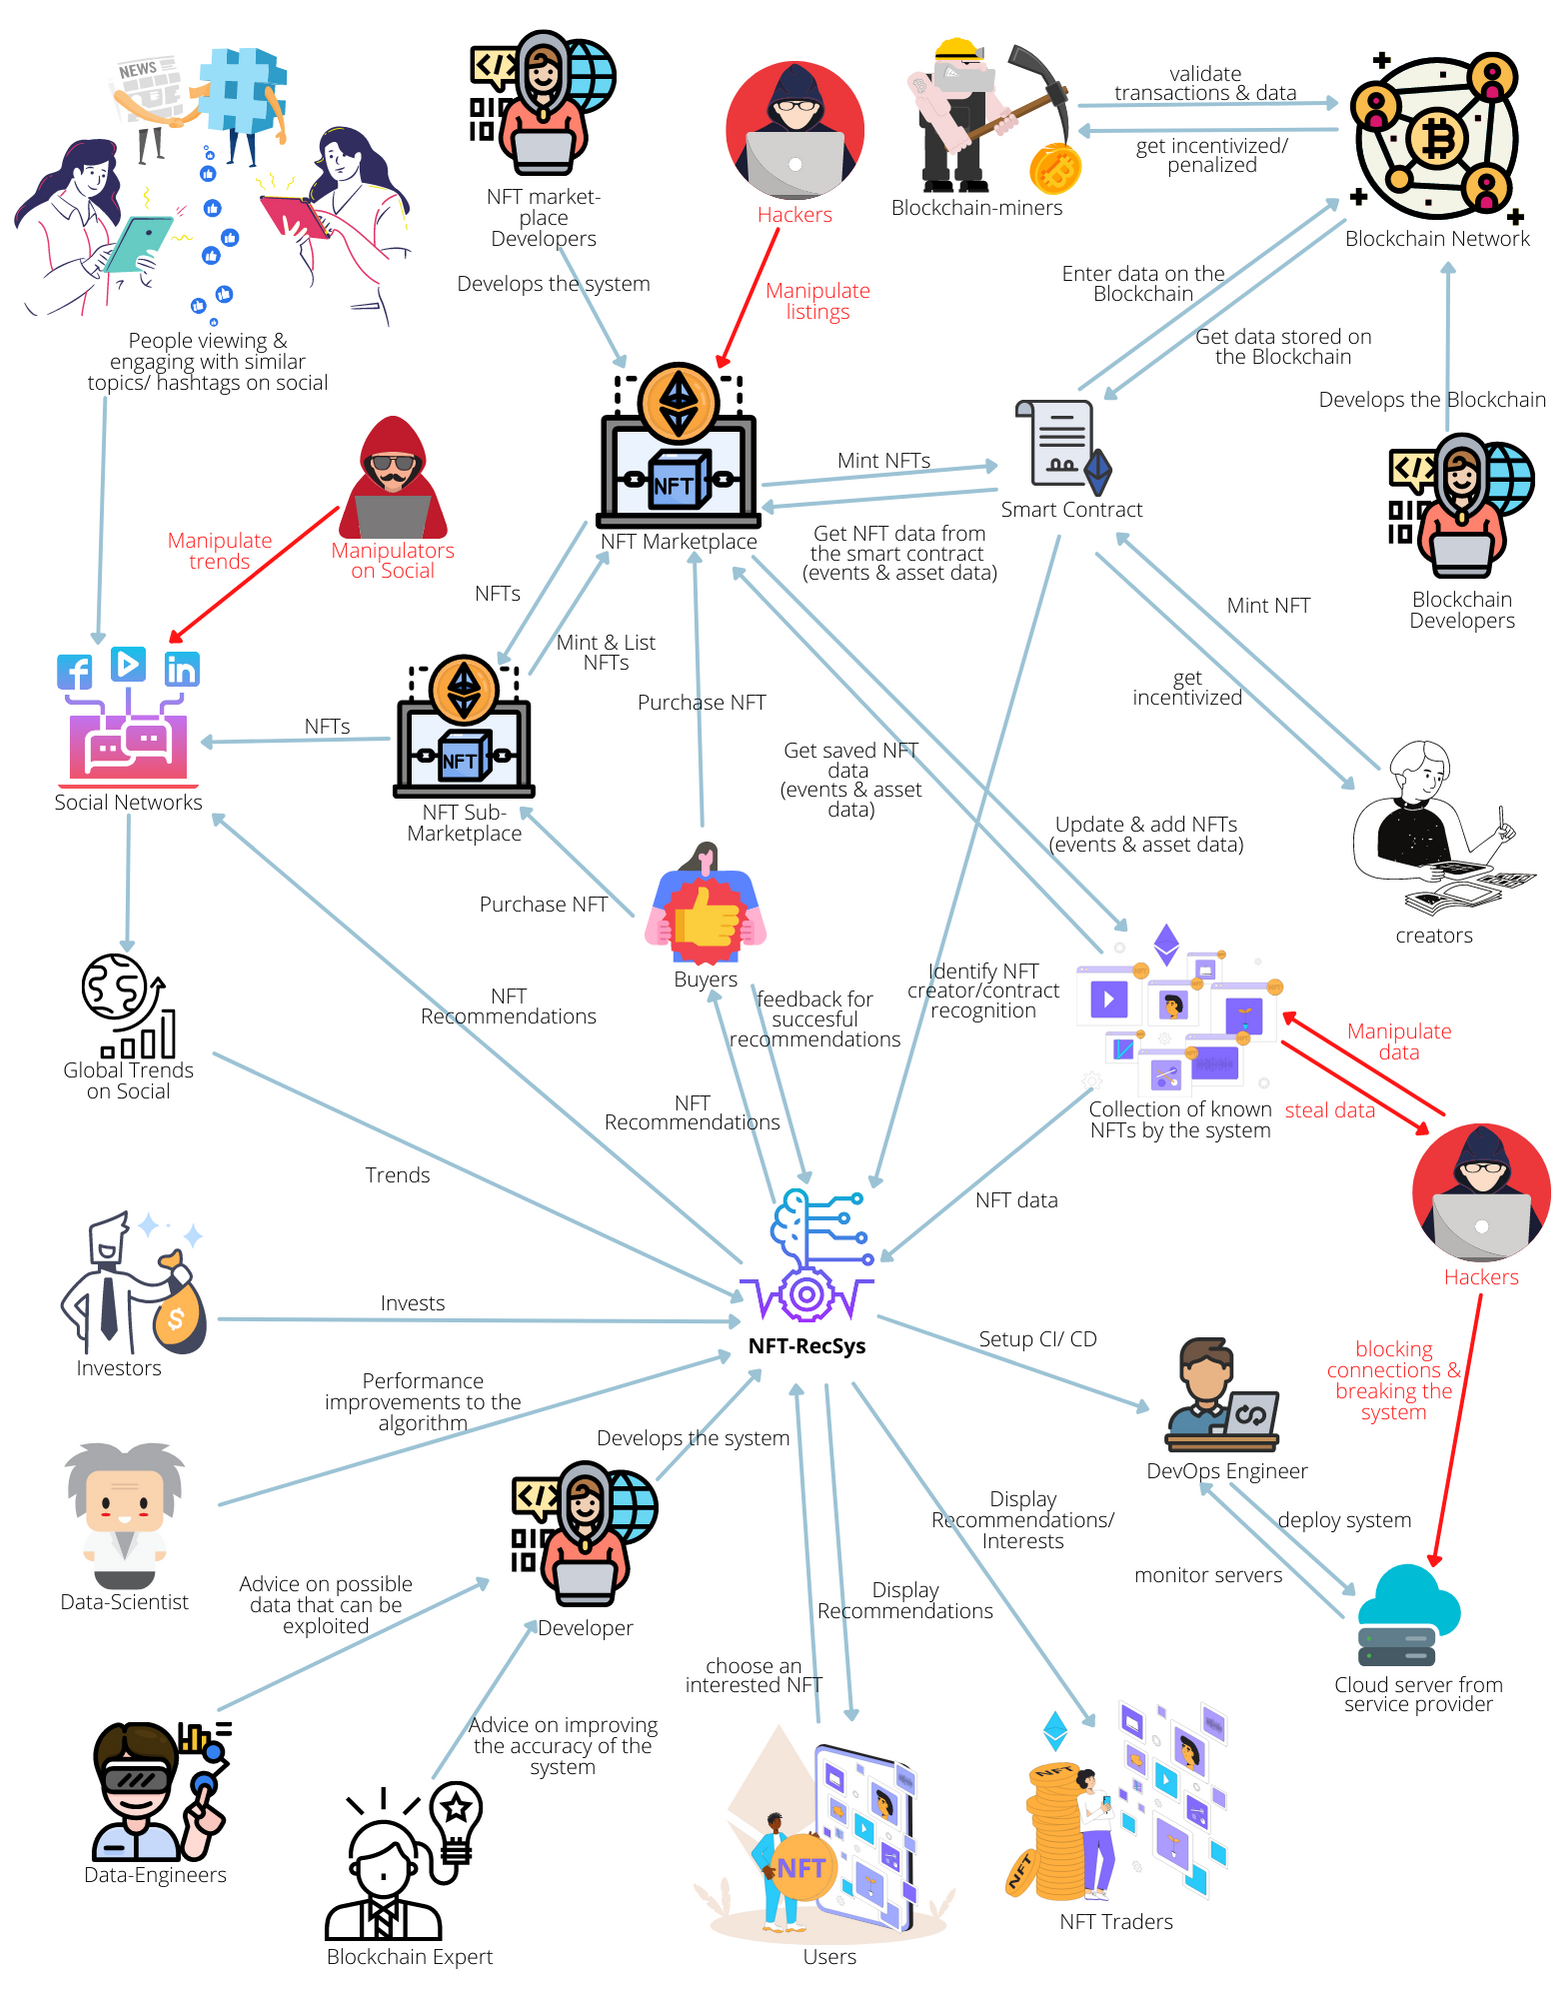
\includegraphics[width=\textwidth]{images/SRS/rich-picture.png}}
\caption{Rich Picture Diagram \textit{(self-composed)}}
\label{fig:rich-picture}
\end{figure}

\section{Stakeholder Analysis}

\subsection{Stakeholder Onion Model}
% would be easier to do this in Figma - drawing circles and stuff

\subsection{Stakeholder Viewpoints}


\section{Requirement Elicitation Methodologies}

\section{Analysis of Data \& Presentation of the Outcome through Elicitation Methodologies}

\section{Summary of Findings}

\section{Context Diagram}

\section{Use Case Diagram}

\section{Use Case Descriptions}

\section{Requirements}

\subsection{Functional Requirements}

\subsection{Non-functional Requirements}

\section{Chapter Summary}
. A Rich Picture Diagram was drawn to understand how the system connects with the society to understand the stakeholders of the system. Saunder's Onion model was used to represent the stakeholders with the flow of influence of each stakeholder. Requirement gathering techniques were utilized to gather all the required data and opinions of possible stakeholders of the system. Lastly, the system's use cases, functional, and non-functional requirements were specified based on the insights derived from the requirement elicitation techniques.